\section{Speech in communication}

This section will analyse speech intelligibility with respect to communication. Speech intelligibility is a wide topic which depend on the speech quality, noise and the frequency range. This section will focus on the speech intelligibility frequency range which might differ from the speech power frequency range. This analysis is done to determined the necessary frequency range in electronic systems for communication. The section will start investigate the production of speech and then the perception of the spoken speech. It will start analyse the speech power frequency range, and then compare it with speech intelligibility and conclude on a necessary frequency range for communication systems.

One on the most important acoustics factor in the human speech is the glottal organ, which make the fundamental frequency of the voice $f_0$. The fundamental frequency is person dependent but the mean differs from male and female and the type of communication e.g. song speech or jelling. For male the mean fundamental frequency for conversational speech is \SI{120}{\hertz} and for female it is \SI{200}{\hertz}. The fact that the fundamental frequency is in the low frequency region does not mean that the transmitted frequency though out the mouth is in only in the low frequency range . The throat speaking system contain a transfer function from the the glottal organ to the output of a mouth  which change the frequency response dramatically \citep{pulkki2015}. The following \autoref{fig:speech_system} shows the path way for the air from the glottal to the lips.

 \begin{figure}[H]
	\centering
		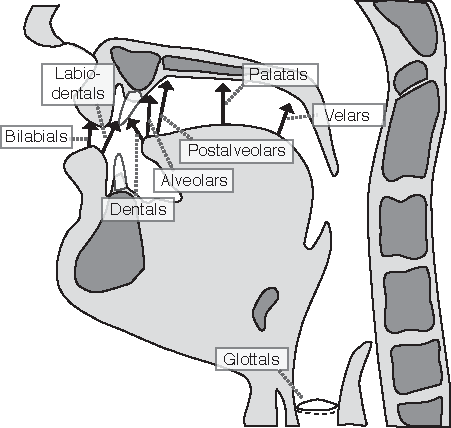
\includegraphics[width=1\textwidth]{glottal}
		\caption{The figure shows the path way from the glottal to the lips \citep{pulkki2015}}
		\label{fig:speech_system}
\end{figure}

The transfer function is human depending or more specific throat, mouth and nose depending. The mean length for the throat from the glottal organ to the lips is \SI{17}{\centi\meter} for male and \SI{14}{\centi\meter} for female. glottal oscillation is mixed with unvoiced airflow in the throat which make turbulence in the transfer of voice. This generate e.g. noise and explosive transient-like sound in the voice output. Another factor is the position of the lips, which act like a radiation filter, e.g. when pronouncing ''O'' the lips have to be shaped specially otherwise the letter sound wrong and if the nose is closed the voice also changed. All those factor for the speech make the frequency range of speech to start below \SI{100}{\hertz} and go upon several \si{\kilo\hertz} \citep{pulkki2015}.The following \autoref{fig:speech_transfer_system} shows a signal block diagram for the speech transfer function.

 \begin{figure}[H]
	\centering
		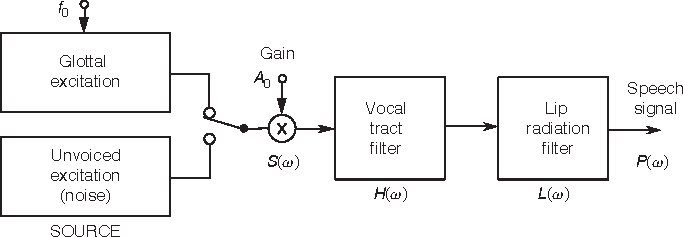
\includegraphics[width=1\textwidth]{speech_transfer}
		\caption{The figure shows a block diagram for the speech transfer function \citep{pulkki2015}}
		\label{fig:speech_transfer_system}
\end{figure}

In language depending speech there is some low frequency component generating by the tongue there goes down to \SI{20}{\hertz}. The tongue is generating the low frequency by trilling e.g. ''r'' in Spanish. The highest frequency component is generated by singing and goes up to \SI{7}{\kilo\hertz} \citep{pulkki2015}. At this point all frequency above \SI{7}{\kilo\hertz} is only harmonic distortion of the voice. The range from \SI{20}{\hertz} to \SI{7}{\kilo\hertz} is then the outer limit but the frequency area might not be that wide when it is the intelligibility that is of important. Filtering away some of the frequency might not affect the speech intelligibility. 

For fully understand what there is needed for good speech intelligibility, the speech intelligibility meaning has to be understood. The speech intelligibility is a measure of how much of a message has been extracted from the recognized phonemes. Phonemes is the smallest unit of speech \citep{arl_us_army}. This measure indicate how good words and sentences can be understood in a listening event. The speech intelligibility  is expressed in percentage of understood speech. The power spectrum of the speech, which earlier was analysed to be within \SI{20}{\hertz} to \SI{7}{\kilo\hertz}, is not correlated to the speech intelligibility. This mean that the understanding of speech might not be in the area of highest speech power. 

Most of the speech power is distributed near the fundamental frequency of the voice, but for speech intelligibility measure this frequency area is below \SI{5}{\percent}. Therefore when hearing speech, the frequency of the voice might not be observed as its fundamental frequency but much higher. in fact \SI{60}{\percent} of the speech intelligibility lays in only \SI{5}{\percent} of the speech power spectrum \citep{arl_us_army}. The spectral centroid of the speech intelligibility frequency are various from language but not fare away from each other. For the English language the centroid is at \SI{1.5}{\kilo\hertz} \citep{arl_us_army}. The following \autoref{fig:speech_intelligibility} shows the power and intelligibility in octave. 

 \begin{figure}[H]
	\centering
		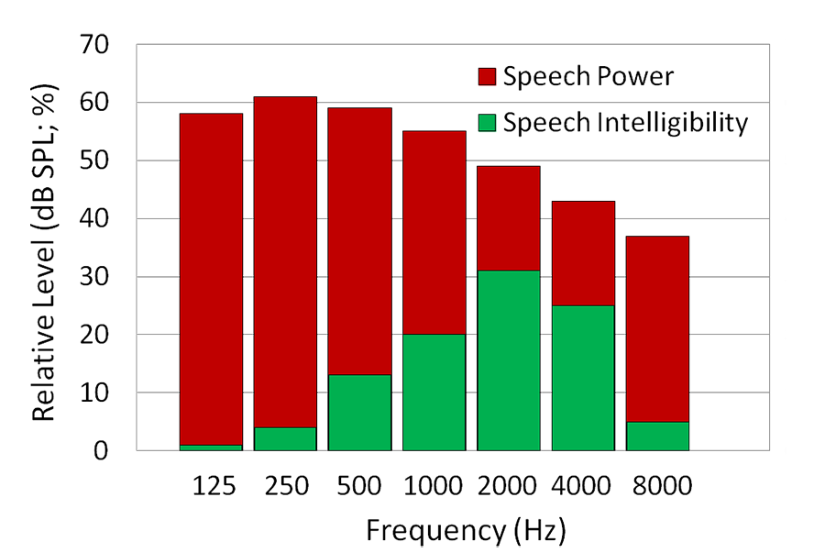
\includegraphics[width=1\textwidth]{speech_intelligibility}
		\caption{The figure shows the power and intelligibility in octave  \citep{arl_us_army}}
		\label{fig:speech_intelligibility}
\end{figure}

As it can be seen at \autoref{fig:speech_intelligibility} the frequency range can be further limited to the range \SI{355}{\hertz} up to \SI{5.68}{\kilo\hertz} because of the outer low frequency limit of the \SI{500}{\hertz} octave band and the upper outer high frequency limit for the \SI{4} octave band. 

In word the vowels and consonants are not equally distributed for speech intelligibility, in fact they are fare away from each other. For speech intelligibility the consonant is the dominant part, and the reason shall be founded in the difference between speech power and speech intelligibility \autoref{fig:speech_intelligibility}. The vowel is actually the letters with the highest power and in the low frequency region, where the consonant is of less power but in higher frequency. With this in mind the consonants is the important for speech intelligibility where vowel do not matter as much.

\subsection{conclusion}
It can be concluded that the transducer shall at less have a good frequency response in the frequency range from \SI{355}{\hertz} up to \SI{5.68}{\kilo\hertz} to establish a good speech intelligibility in a communication system.

